\documentclass[aspectratio=169]{beamer}

% <<< BEGIN tema

\usetheme[nomyriadpro,progressbar]{unam}

% logos (los valores por defecto ya apuntan a assets/; se pueden cambiar aquí)
\unammotto{}
\unamslidelogo{
\includegraphics[width=0.45\paperheight]{assets/unam-escudo-gris}}

% portada: escudo más grande, ocupando el espacio sobre el título
\unamtitlelogo{
\includegraphics[height=0.5\paperheight]{assets/unam-escudo-gris}}
\unamtitlelogoshift{-0.3cm}
% pie de página: GitHub en lugar de www.unam.mx
\unamurl{https://github.com/jairferrara}{github.com/jairferrara}

% presentación final: se usan las diapositivas separadoras de sección del tema
% (versión propuesta: \AtBeginSection{} las desactivaba)
% título largo: fuente un poco más chica en la portada
\setbeamerfont{title}{size=\large, series=\bfseries}

% sin símbolos de navegación
\beamertemplatenavigationsymbolsempty

% cómo se muestran los elementos ocultos: invisible / transparent / dynamic
\setbeamercovered{transparent}
\setbeamersize{text margin left=1.2em,text margin right=1.2em}
\addtobeamertemplate{frametitle}{}{\vspace{0.2em}}

% >>> END

% <<< BEGIN paquetes y macros

\usepackage{amsmath,amssymb,mathtools}
\usepackage{physics}
\usepackage{bm}
\usepackage{booktabs}
\usepackage{xcolor}
\usepackage{hyperref}
\usepackage{multimedia}
\usepackage{appendixnumberbeamer} % respaldo fuera del conteo de diapositivas
\usepackage[utf8]{inputenc}
\usepackage[T1]{fontenc}
\DeclareFontShape{T1}{cmss}{b}{n}{<->ssub*cmss/bx/n}{}
\DeclareFontShape{T1}{cmss}{m}{sc}{<->ssub*cmr/m/sc}{}

% gráficos con TikZ
\usepackage{tikz}
\usetikzlibrary{fit, backgrounds, arrows.meta, positioning, shadows}

% pendientes: \todo[inline]{...}, \missingfigure{...} y \postit{...}
% Versión final: \usepackage[disable]{todonotes} y desaparecen todos (también los post-its).
\usepackage[colorinlistoftodos]{todonotes}
\setuptodonotes{color=orange!35, bordercolor=orange!70!black, size=\footnotesize}
\tikzset{pendiente/.style={fill=orange!35, draw=orange!70!black, rounded corners=2pt,
  font=\footnotesize, text=black, align=left, inner sep=5pt}}
\tikzset{postit/.style={fill=yellow!65, draw=yellow!45!orange, text width=4.4cm,
  align=left, inner sep=9pt, rotate=-4, font=\small\sffamily, text=black!85,
  drop shadow={opacity=0.35}}}
% \postit[<estilo tikz>]{<texto>}: nota adhesiva en la esquina superior derecha de la página.
% Se registra en la lista de pendientes igual que un \todo y obedece la opción disable.
\makeatletter
\newcommand{\postit}[2][]{%
  \if@todonotes@disabled\else
    \begin{tikzpicture}[remember picture, overlay]
      \node[postit, anchor=north east, #1]
        at ([xshift=-0.6cm, yshift=-0.6cm]current page.north east) {#2};
    \end{tikzpicture}%
    \addcontentsline{tdo}{todo}{\fcolorbox{yellow!45!orange}{yellow!65}%
      {\textcolor{yellow!65}{o}}\ #2}%
  \fi}
% \siPendientes{...}: solo se dibuja si todonotes no está en modo disable (p.ej. notas en TikZ).
\newcommand{\siPendientes}[1]{\if@todonotes@disabled\else#1\fi}
% \listapendientes: índice de todos los pendientes (\todo, \postit, \registrarPendiente) con su página.
% Se usa dentro de un frame porque \listoftodos hace un \section*, que choca con Beamer.
\newcommand{\listapendientes}{\@starttoc{tdo}}
% \registrarPendiente{<texto>}: agrega <texto> a la lista de pendientes (para notas hechas a mano).
\newcommand{\registrarPendiente}[1]{\if@todonotes@disabled\else
  \addcontentsline{tdo}{todo}{\fcolorbox{orange!70!black}{orange!35}%
    {\textcolor{orange!35}{o}}\ #1}\fi}
\makeatother

% carpeta de imágenes
\graphicspath{{images/}{../reporte/images/}}   % las figuras de resultados son las mismas del reporte

\definecolor{myblue}{RGB}{30,100,180}
\definecolor{myred}{RGB}{180,30,30}
\definecolor{mygreen}{RGB}{20,140,60}
\definecolor{mypurple}{RGB}{120,30,160}
\definecolor{myorange}{RGB}{220,120,0}

% macros de ejemplo (agregar las propias del proyecto aquí)
\newcommand{\kv}{\mathbf{k}}
\newcommand{\etal}{\textit{et al.}}

% >>> END

% <<< BEGIN metadatos

\title[Estimadores de $\xi(r)$ y dilución de materia oscura]{Estudio sobre los estimadores de la función de correlación para modelos de dilución de materia oscura}
\subtitle[Propuesta de proyecto final]{Propuesta de proyecto final}
\author[J. Ferrara]{Jair Ferrara}
\institute{Universidad Nacional Autónoma de México}
\date{18 de noviembre de 2026}

% >>> END

\newcommand{\DD}{\mathrm{DD}}
\newcommand{\DR}{\mathrm{DR}}
\newcommand{\RR}{\mathrm{RR}}

\newcommand{\dil}[1]{\textcolor{myred}{#1}}   % términos nuevos por dilución

\begin{document}

\titleframe[\postit{\textbf{TODO:} elegir y actualizar el título del beamer
  (también el subtítulo y la fecha).}]

% índice de pendientes: no cuenta en la numeración y desaparece con [disable]
\siPendientes{%
\begin{frame}[noframenumbering]{Pendientes}
  \small
  \listapendientes
\end{frame}}

% ####################################################################
% ##########  VERSIÓN FINAL (presentación del proyecto)  ##############
% ####################################################################

% ====================================================
\section{Motivación}
% ====================================================

\begin{frame}{Motivación}
  \begin{columns}[c]
    \begin{column}{0.56\textwidth}
      \centering
      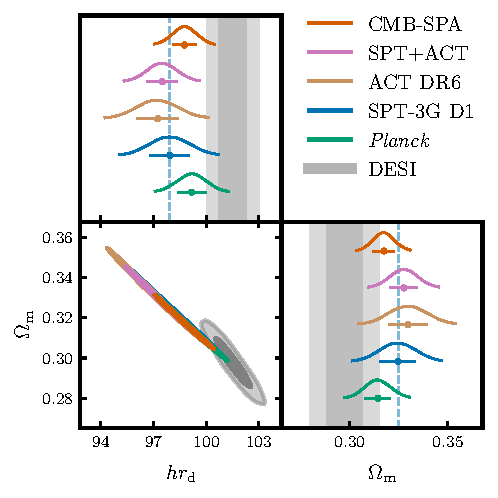
\includegraphics[height=0.74\paperheight]{spt3g_fig25_hord}
    \end{column}
    \begin{column}{0.42\textwidth}
      El BAO de \textbf{DESI DR2} prefiere un $\Omega_m$ menor que el CMB:
      $2.0$--$3.7\sigma$ en $\Lambda$CDM.

      \vspace{1.5em}
      {\scriptsize Fig.~25 de E.~Camphuis \etal\ (SPT-3G D1),\\ arXiv:2506.20707.}

      \vspace{1em}
      \todo[inline]{Incluir una motivación para el trabajo estadístico y para el modelo cosmológico.}
      \todo[inline]{Averiguar si lo que se ve de DESI en la figura de Camphuis es solo BAO o \emph{full shape}.}
    \end{column}
  \end{columns}
\end{frame}

% ====================================================
\section{Punto de partida}
% ====================================================

% ---- 1. continuidad ----
\begin{frame}{Continuidad}
  \begin{columns}[c]
    \begin{column}{0.49\textwidth}
      \centering
      {\LARGE
      \[
        \dot\rho + 3H\rho + \tfrac1a\nabla\!\cdot(\rho\,\mathbf v) = 0
      \]}
      \vspace{0.2em}
      {\LARGE\textcolor{UNAMGold}{$\Downarrow$}}
      \vspace{0.4em}
      {\large
      \begin{gather*}
        \dot\delta + \tfrac1a\nabla\!\cdot\big[(1+\delta)\,\mathbf v\big] = 0\\[1.0em]
        \dot{\mathbf v} + H\mathbf v + \tfrac1a(\mathbf v\!\cdot\!\nabla)\mathbf v = -\tfrac1a\nabla\Phi\\[1.0em]
        \nabla^2\Phi = \tfrac32\,\Omega_m H^2 a^2\,\delta
      \end{gather*}}
    \end{column}
    \vrule
    \begin{column}{0.49\textwidth}
      \centering
      {\LARGE
      \[
        \dot\rho + 3H\rho + \tfrac1a\nabla\!\cdot(\rho\,\mathbf v) = \dil{S}
      \]}
      \vspace{0.2em}
      {\LARGE\textcolor{UNAMGold}{$\Downarrow$}}
      \vspace{0.4em}
      {\large
      \begin{gather*}
        \dot\delta + \tfrac1a\nabla\!\cdot\big[(1+\delta)\,\mathbf v\big] = \dil{\frac{S-(1+\delta)\bar S}{\bar\rho}}\\[1.0em]
        \dot{\mathbf v} + H\mathbf v + \tfrac1a(\mathbf v\!\cdot\!\nabla)\mathbf v = -\tfrac1a\nabla\Phi\\[1.0em]
        \nabla^2\Phi = \tfrac32\,\Omega_m H^2 a^2\,\delta
      \end{gather*}}
    \end{column}
  \end{columns}
\end{frame}

% ---- 2. densidad vs. perturbación ----
\begin{frame}{¿$S\propto\rho$ o $S\propto\delta$?}
  \centering
  \begin{block}{}
    \centering\large
    $\displaystyle \dot\delta + \tfrac1a\nabla\!\cdot\big[(1+\delta)\,\mathbf v\big]
      = \frac{S - (1+\delta)\,\bar S}{\bar\rho}$
  \end{block}

  \vspace{1.0em}
  {\large
  \begin{tabular}{c@{\hspace{2.5cm}}c}
    $S=\Gamma\rho$, \ $\bar S=\Gamma\bar\rho$ & $S=-gH\bar\rho\,\delta$, \ $\bar S=0$\\[0.6em]
    $\Downarrow$ & $\Downarrow$\\[0.4em]
    $\dfrac{S-(1+\delta)\bar S}{\bar\rho} = 0$ & $\dfrac{S-(1+\delta)\bar S}{\bar\rho} = \dil{-gH\delta}$
  \end{tabular}}

  \vspace{0.5em}
  {\footnotesize $\Gamma$: tasa de interacción (energía oscura interactuante)}

\end{frame}

% ---- 3. toy model ----
\begin{frame}{Toy model}
  \begin{columns}[c]
    \begin{column}{0.46\textwidth}
      \[
        g(z) = \frac{g_0}{2}\left[1 - \tanh\!\left(\frac{z-z_t}{\Delta z}\right)\right]
      \]
      \vspace{0.3em}
      \begin{itemize}
        \setlength\itemsep{0.6em}
        \item $z\gg z_t$: \ $g\to0$ \ ($\Lambda$CDM)
        \item $z\ll z_t$: \ $g\to g_0$ \ (dilución)
      \end{itemize}
      \vspace{0.8em}
      \begin{alertblock}{}
        \centering
        Fondo $\Lambda$CDM fijo: aísla el efecto de la dilución en el \emph{clustering}.
      \end{alertblock}
    \end{column}
    \begin{column}{0.52\textwidth}
      \centering
      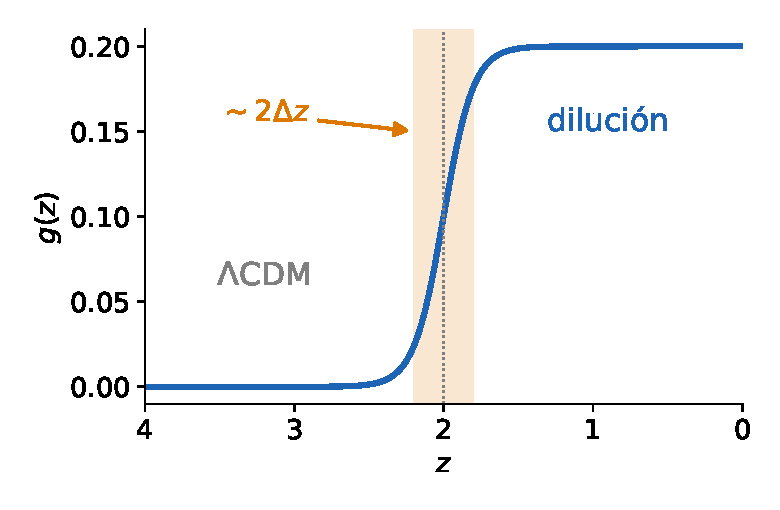
\includegraphics[width=\linewidth]{toy_gz}\\[-0.2em]
      {\footnotesize $g_0=0.2$, \ $z_t=2$, \ $\Delta z=0.2$, \ $\Omega_{m0}=0.3$}
    \end{column}
  \end{columns}
\end{frame}

% ---- 4. tres casos (fotos de la animación) ----
% Panel: #1 amplitud A, #2 media R, #3 A de referencia, #4 R de referencia (vacíos: sin referencia), #5 etiqueta.
% En punteado gris: el estado ΛCDM inicial, para ver qué cambia con la dilución.
\newcommand{\dilpanel}[5]{%
  \begin{tikzpicture}[x=0.45cm, y=1.3cm,
      declare function={dl(\x,\a)=\a*(0.8*sin(60*\x)+0.45*sin(140*\x+60));}]
    \node[font=\large, text=UNAMDarkBlue] at (5,2.3) {#5};
    \fill[UNAMLightBlue!25] (0,0) -- plot[domain=0:10, samples=100] (\x,{#2*(1+dl(\x,#1))}) -- (10,0) -- cycle;
    \ifx\relax#3\relax\else
      \draw[black!55, thick, dashed] plot[domain=0:10, samples=100] (\x,{#4*(1+dl(\x,#3))});
    \fi
    \draw[UNAMDarkBlue, very thick] plot[domain=0:10, samples=100] (\x,{#2*(1+dl(\x,#1))});
    \draw[UNAMGold, thick] (0,#2) -- (10,#2) node[right, font=\small] {$\bar\rho$};
    \draw[gray] (0,0) -- (10,0);
    \node[left] at (0,1) {$\rho$};
    \begin{scope}[yshift=-1.6cm, y=1.3cm]
      \draw[gray] (0,0) -- (10,0);
      \ifx\relax#3\relax\else
        \draw[black!55, thick, dashed] plot[domain=0:10, samples=100] (\x,{dl(\x,#3)});
      \fi
      \draw[UNAMLightBlue, very thick] plot[domain=0:10, samples=100] (\x,{dl(\x,#1)});
      \node[left] at (0,0) {$\delta$};
    \end{scope}
  \end{tikzpicture}}

\begin{frame}{Tres casos}
  \centering
  \vspace{0.8em}
  \resizebox{\textwidth}{!}{%
    \dilpanel{0.5}{1}{}{}{$S=0$}\hspace{0.8cm}%
    \dilpanel{0.5}{0.6}{0.5}{1}{$S=\Gamma\rho,\ \Gamma<0$}\hspace{0.8cm}%
    \dilpanel{0.25}{1}{0.5}{1}{$S=-gH\bar\rho\,\delta$}}

  \vspace{0.4em}
  \todo[inline]{Hacer pruebas cambiando $g_0$, $z_t$ y $\Delta z$ para ver cómo afectan los resultados.}
\end{frame}

% ---- 5. ecuaciones a resolver ----
\begin{frame}{Crecimiento lineal}
  \centering
  {\Large
  \begin{gather*}
    \ddot D_+ + (2+g)\,H\dot D_+ - \Big[\tfrac32\Omega_m H^2 - g\,(2H^2+\dot H) - \dot g\,H\Big] D_+ = 0
  \end{gather*}}
  \vspace{0.2em}
  {\LARGE\textcolor{UNAMGold}{$\Downarrow$}}
  \vspace{0.6em}

  \begin{minipage}{0.62\linewidth}
    \begin{block}{}
      \centering\large
      $\displaystyle P_{\rm dil}(k,z) = \left[\frac{D_+(z)}{D_+^{\Lambda{\rm CDM}}(z)}\right]^2 P_L(k,z)$
    \end{block}
  \end{minipage}
\end{frame}

% ====================================================
\section{Objetivo}
% ====================================================

% ---- 1. diagrama de flujo ----
\begin{frame}{Flujo de trabajo}
  \centering
  \vspace{1.2em}
  \resizebox{\textwidth}{!}{%
  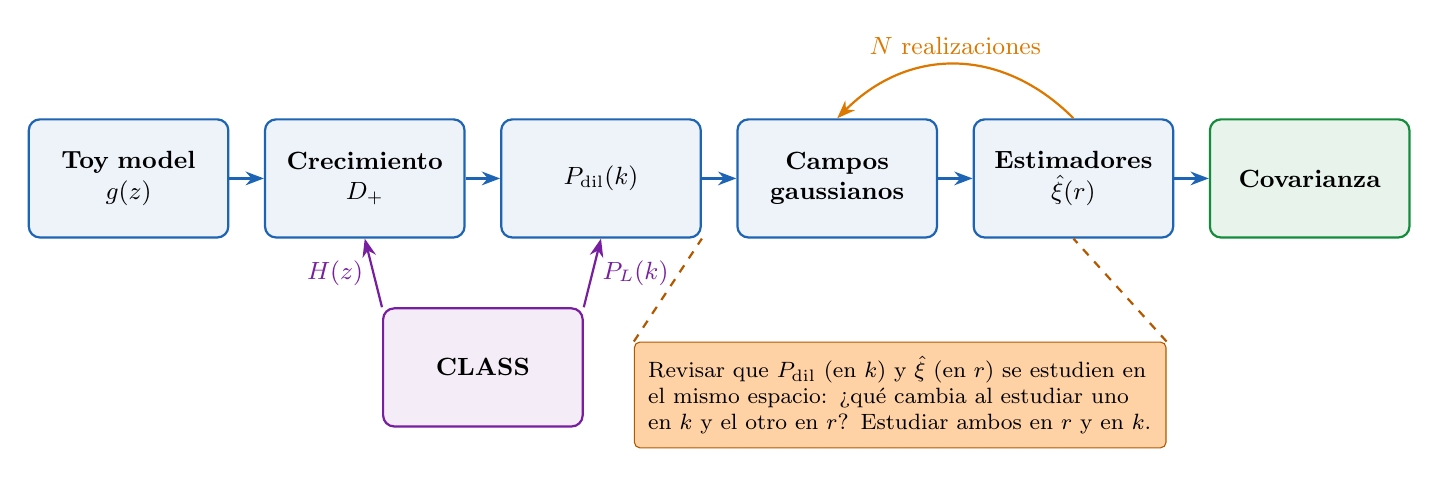
\begin{tikzpicture}[
      box/.style={draw=myblue, thick, rounded corners, fill=myblue!8,
        align=center, minimum height=1.5cm, text width=2.3cm, font=\small},
      ext/.style={box, draw=mypurple, fill=mypurple!8},
      res/.style={box, draw=mygreen, fill=mygreen!10},
      arr/.style={-{Stealth}, thick, myblue}]
    \node[box] (toy)   at (0,0)    {\textbf{Toy model}\\$g(z)$};
    \node[box] (ode)   at (3,0)    {\textbf{Crecimiento}\\$D_+$};
    \node[box] (pdil)  at (6,0)    {$P_{\rm dil}(k)$};
    \node[ext] (class) at (4.5,-2.4) {\textbf{CLASS}};
    \node[box] (field) at (9,0)    {\textbf{Campos gaussianos}};
    \node[box] (est)   at (12,0)   {\textbf{Estimadores}\\$\hat\xi(r)$};
    \node[res] (cov)   at (15,0)   {\textbf{Covarianza}};
    \draw[arr] (toy) -- (ode);
    \draw[arr] (ode) -- (pdil);
    \draw[arr] (pdil) -- (field);
    \draw[arr] (field) -- (est);
    \draw[arr] (est) -- (cov);
    \draw[arr, mypurple] (class.north west) -- node[left, font=\small] {$H(z)$} (ode.south);
    \draw[arr, mypurple] (class.north east) -- node[right, font=\small] {$P_L(k)$} (pdil.south);
    \draw[-{Stealth}, thick, myorange] (est.north) to[out=135, in=45, looseness=1.1]
      node[above, font=\small] {$N$ realizaciones} (field.north);
    \siPendientes{%
      \node[pendiente, text width=6.4cm] (tdk) at (9.8,-2.75)
        {Revisar que $P_{\rm dil}$ (en $k$) y $\hat\xi$ (en $r$) se estudien en el mismo
         espacio: ¿qué cambia al estudiar uno en $k$ y el otro en $r$? Estudiar ambos en $r$ y en $k$.};
      \draw[orange!70!black, thick, dashed] (tdk.north west) -- (pdil.south east);
      \draw[orange!70!black, thick, dashed] (tdk.north east) -- (est.south);}
  \end{tikzpicture}}
  \registrarPendiente{Revisar que $P_{\rm dil}$ ($k$) y $\hat\xi$ ($r$) se estudien en el mismo
    espacio; estudiar ambos en $r$ y en $k$.}
\end{frame}

% ---- 2. qué se busca ----
\begin{frame}{Objetivo}
  Comparar la covarianza de $\hat\xi(r)$ obtenida con distintos estimadores,
  en $\Lambda$CDM y con dilución.
  \vspace{1em}
  \begin{enumerate}
    \setlength\itemsep{0.9em}
    \item \textbf{Campos gaussianos} con $P_{\rm dil}(k)$, para $g_0=0$ y $g_0=0.2$.
    \item Medir $\hat\xi(r)$ con Peebles--Hauser, Davis--Peebles, Hamilton y Landy--Szalay
      en $N$ realizaciones.
    \item Calcular la covarianza de cada estimador.
    \item Comparar las covarianzas entre estimadores y entre modelos.
  \end{enumerate}
\end{frame}

% ====================================================
\section{Entradas y salidas}
% ====================================================

\begin{frame}{Entradas}
  \begin{itemize}
    \setlength\itemsep{1.4em}
    \item \textbf{CLASS:} \ $P_L(k)$ \ y el fondo \ $H(z)$, $\Omega_m(z)$.
    \item \textbf{Toy model:} \
      $\displaystyle g(z) = \frac{g_0}{2}\left[1 - \tanh\!\left(\frac{z-z_t}{\Delta z}\right)\right]$
    \item \textbf{Caja periódica:} \ $L=1000\,h^{-1}$Mpc, \ malla $128^3$.
    \item \textbf{$N$ realizaciones} \ por modelo, \ con catálogos aleatorios para los estimadores.
  \end{itemize}
\end{frame}

\begin{frame}{Salidas}
  \begin{itemize}
    \setlength\itemsep{1.4em}
    \item $D_+(z)$ \ y \ $P_{\rm dil}(k)$.
    \item $\hat\xi(r)$ \ de cada estimador en cada realización.
    \item $\hat C_{ij}$ \ y su matriz de correlación, \ por estimador y por modelo.
    \item Comparación de las varianzas entre estimadores.
  \end{itemize}
\end{frame}

% ====================================================
\section{Pseudocódigo}
% ====================================================

\newcommand{\kw}[1]{\textcolor{UNAMDarkBlue}{\textbf{#1}}}
\newcommand{\cm}[1]{\textcolor{black!50}{\##1}}
\begin{frame}{Algoritmo}
  \centering
  \begin{tikzpicture}
    \node[fill=black!3, inner sep=9pt, text width=0.86\textwidth,
          font=\ttfamily, align=left] (code) {%
      cosmo = CLASS(cosmología)                    \cm{ P\_L(k), H(z)}\\
      R = aleatorios($\alpha$);  RR = contar\_pares(R)   \cm{ R fijo}\\
      \kw{for} g0 \kw{in} [0, 0.2]:\\
      \hspace*{2em}Dp = crecimiento(g0, cosmo)\\
      \hspace*{2em}Pdil = (Dp / Dp\_LCDM)**2 * P\_L\\
      \hspace*{2em}\kw{for} s \kw{in} 1..N:\\
      \hspace*{4em}D = puntos(campo\_gaussiano(Pdil, s))\\
      \hspace*{4em}DD, DR = contar\_pares(D, R)\\
      \hspace*{4em}\kw{for} est \kw{in} [PH, DP, Ham, LS]:\\
      \hspace*{6em}xi[g0, est, s] = est(DD, DR, RR)\\
      \hspace*{2em}C[g0, est] = cov(xi[g0, est, :])     \cm{ para cada est}\\
      comparar(C)};
    \fill[UNAMGold] (code.north west) rectangle ([xshift=4pt]code.south west);
  \end{tikzpicture}
\end{frame}

% ====================================================
\section{Resultados esperados}
% ====================================================

\begin{frame}{Expectativas}
  \begin{itemize}
    \setlength\itemsep{1.0em}
    \item $\xi_{\rm dil}(r)\simeq0.8\,\xi_{\Lambda{\rm CDM}}(r)$ en $z=0.5$.
      \begin{itemize}
        \item La dilución solo suprime la amplitud, $\big(D_+^{\rm dil}/D_+^{\Lambda{\rm CDM}}\big)^2$:
          misma forma y mismo pico BAO.
      \end{itemize}
    \item La covarianza baja con la amplitud.
      \begin{itemize}
        \item La parte de varianza cósmica escala como $(P_{\rm dil}/P_{\Lambda{\rm CDM}})^2\approx0.64$;
          el ruido de Poisson $1/\bar n$ no se diluye, así que la reducción total es menor.
      \end{itemize}
    \item Diferencias entre estimadores.
      \begin{itemize}
        \item Con R fijo, RR no aporta varianza, solo sesgo; el ruido de DR entra distinto en cada
          estimador. Se compara variando $\alpha=N_R/N_D$.
      \end{itemize}
  \end{itemize}
\end{frame}

% ====================================================
\section{Resultados}
% ====================================================
% Figuras de la corrida con N = 5x10^4 por modelo (las genera covarianza.ipynb en reporte/images/).

\begin{frame}{$\langle\hat\xi(r)\rangle$}
  \centering
  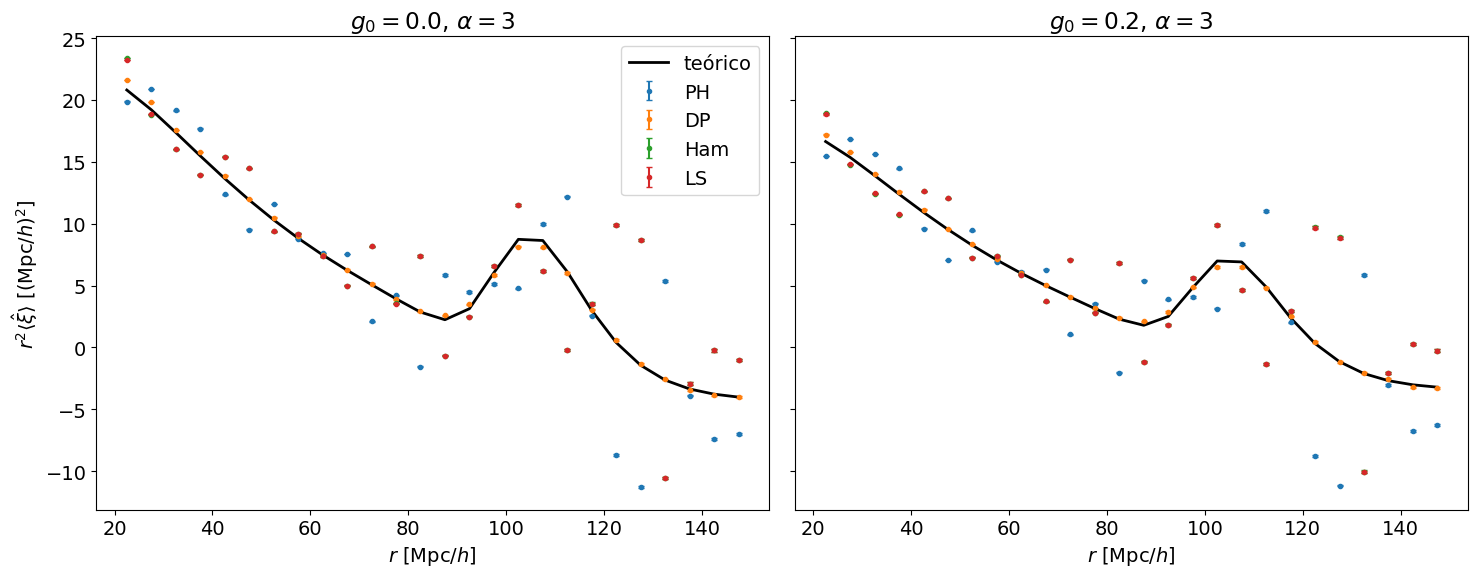
\includegraphics[width=\textwidth, height=0.78\textheight, keepaspectratio]{xi_promedio}
\end{frame}

\begin{frame}{Correlación}
  \centering
  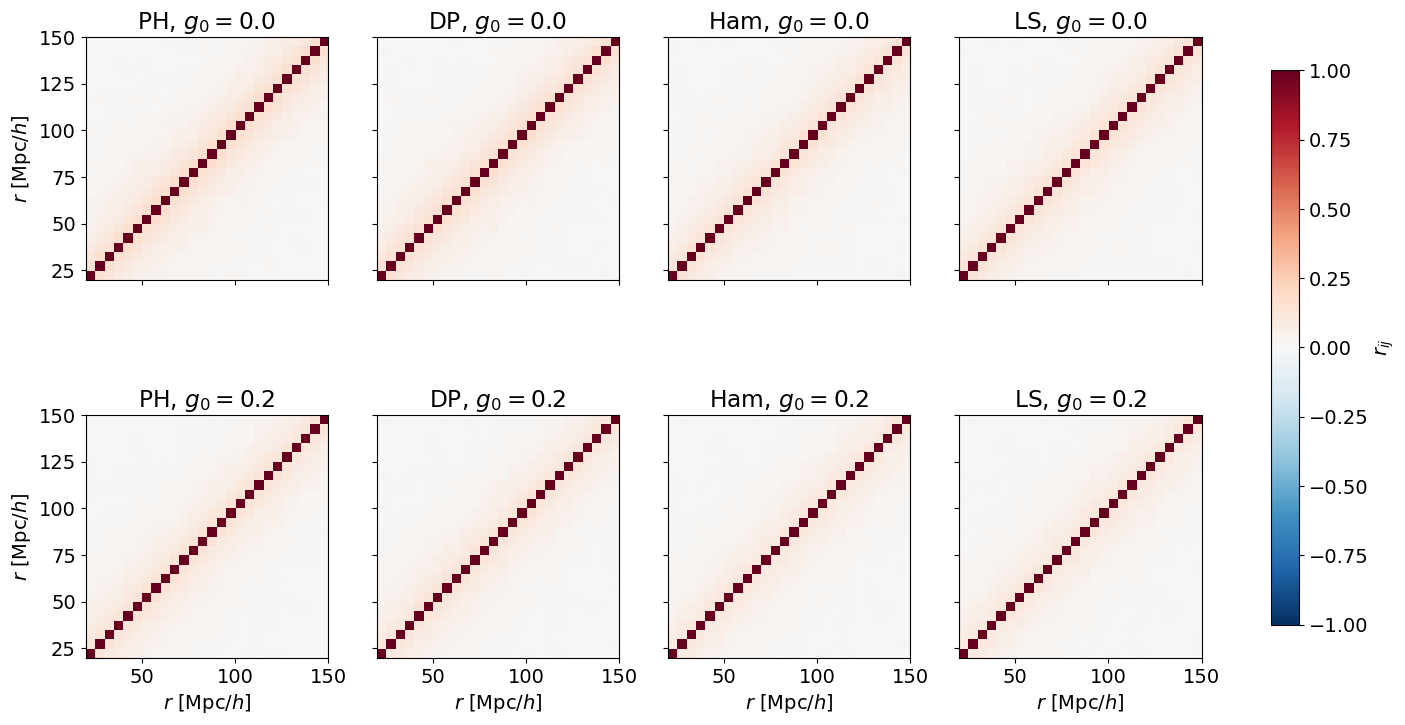
\includegraphics[width=\textwidth, height=0.78\textheight, keepaspectratio]{matrices_correlacion}
\end{frame}

\begin{frame}{Estimadores}
  \centering
  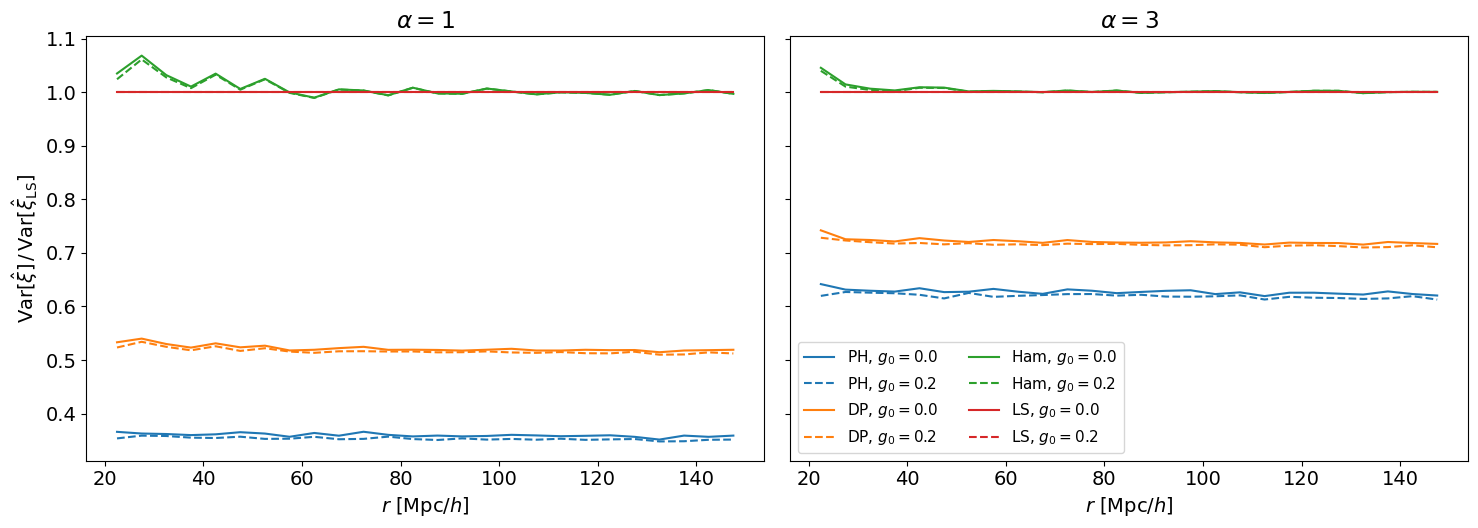
\includegraphics[width=\textwidth, height=0.78\textheight, keepaspectratio]{varianza_estimadores}
\end{frame}

\begin{frame}{Dilución}
  \centering
  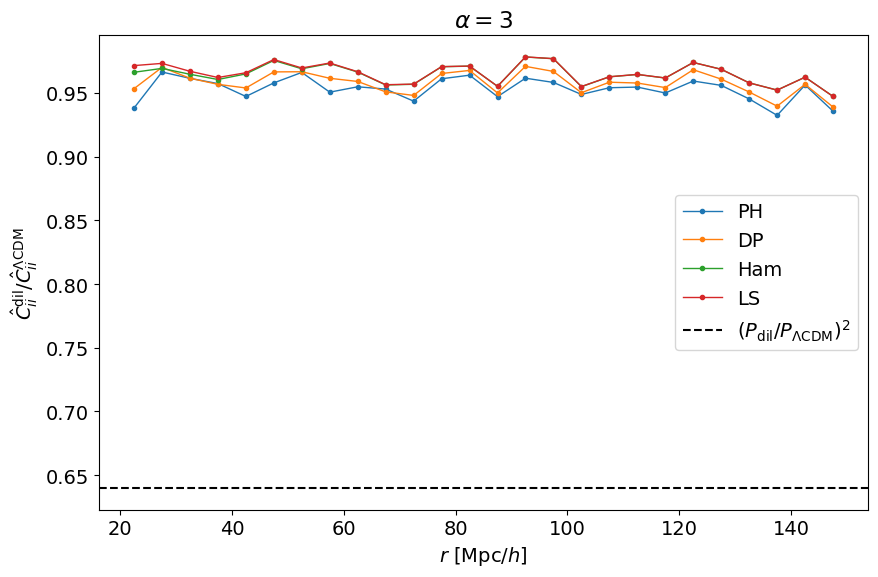
\includegraphics[width=\textwidth, height=0.78\textheight, keepaspectratio]{cociente_modelos}
\end{frame}

% ====================================================
\section{Bibliografía}
% ====================================================

\begin{frame}{Bibliografía}
  \scriptsize
  \begin{block}{Trabajo base}
    \begin{itemize}
      \item A.~Avilés \& J.~Ferrara, \textit{Dark Matter Dilution: A Two-Field Lagrangian
        Perturbation Theory of Large-Scale Structure}, borrador (en preparación).
    \end{itemize}
  \end{block}
  \begin{exampleblock}{Motivación}
    \begin{itemize}
      \item E.~Camphuis \etal\ (SPT-3G), \textit{SPT-3G D1: CMB temperature and polarization
        power spectra and cosmology\ldots}, arXiv:2506.20707.
      \item E.~Silva, G.~Hartmann \& R.~C.~Nunes, \textit{One-loop power spectrum corrections in
        interacting dark energy cosmologies}, PRD \textbf{113} (2026) 063548.
      \item X.~Chen \& A.~Loeb, \textit{Evolving Dark Energy or Evolving Dark Matter?},
        JCAP \textbf{07} (2025) 059.
      \item J.~Khoury, M.-X.~Lin \& M.~Trodden, \textit{Apparent $w<-1$ and a Lower $S_8$ from
        Dark Axion and Dark Baryons Interactions}, PRL \textbf{135} (2025) 181001.
      \item M.~A.~Sabogal, S.~Vagnozzi \& E.~Di Valentino, \textit{Cosmological anatomy of
        interacting dark energy}, arXiv:2609.18288.
    \end{itemize}
  \end{exampleblock}
\end{frame}

% ---- cierre: con fondo de sección ----
\section{¡Gracias! \texorpdfstring{\\[0.4em]}{} {\normalsize ¿Preguntas y comentarios?}}

% ====================================================
% Respaldo: no cuenta en el tiempo ni en el número total de diapositivas
% ====================================================
\appendix
\section{Diapositivas de respaldo}

\begin{frame}{Estimadores de $\xi(r)$}
  Con $N_D$ datos y $N_R=\alpha N_D$ aleatorios; \ DD, DR, RR normalizados por el número de pares:
  \begin{align*}
    \hat\xi_{\rm PH}  &= \frac{\DD}{\RR}-1 &
    \hat\xi_{\rm DP}  &= \frac{\DD}{\DR}-1\\[0.3em]
    \hat\xi_{\rm Ham} &= \frac{\DD\cdot\RR}{\DR^2}-1 &
    \hat\xi_{\rm LS}  &= \frac{\DD-2\DR+\RR}{\RR}
  \end{align*}
  \begin{itemize}
    \item LS y Hamilton cancelan a primer orden la fluctuación de la densidad media y los efectos de borde.
    \item En caja periódica no hay bordes: la ventaja de LS no está garantizada.
    \item Con aleatorios finitos, $\RR$ y $\DR$ añaden ruido: por eso se varía $\alpha$.
  \end{itemize}
\end{frame}

\begin{frame}{Covarianza muestral}
  \[
    \hat C_{ij} = \frac{1}{N-1}\sum_{s=1}^{N}
    (\hat\xi_{s,i}-\bar\xi_i)(\hat\xi_{s,j}-\bar\xi_j),
    \qquad
    r_{ij} = \frac{\hat C_{ij}}{\sqrt{\hat C_{ii}\hat C_{jj}}}
  \]
  \begin{itemize}
    \setlength\itemsep{0.6em}
    \item Una sola caja da un $\hat\xi$; la covarianza es la dispersión entre realizaciones.
    \item El error relativo de la diagonal es $\sigma(\hat C_{ii})/C_{ii}\simeq\sqrt{2/(N-1)}$.
  \end{itemize}
\end{frame}

\begin{frame}{Campos gaussianos}
  \begin{itemize}
    \setlength\itemsep{0.8em}
    \item Campo gaussiano: \
      $\delta(\mathbf k) = \sqrt{P(k)/V_{\rm celda}}\;\mathrm{FFT}[w](\mathbf k)$, \ $w$ ruido blanco real en la malla.
    \item Puntos: Poisson con media \ $\bar n\,V_{\rm celda}\,e^{\delta-\sigma^2/2}$ \ por celda.
    \item Toda su estadística está en $P(k)$ (o en $\xi$):
      \[
        \xi(r) = \int_0^\infty \frac{k^2\,dk}{2\pi^2}\,P(k)\,j_0(kr).
      \]
    \item A orden lineal y a un $z$ fijo, la dilución solo reescala $P$: degenerada con $\sigma_8$.
  \end{itemize}
\end{frame}

% Animación del toy model como video (pympress la reproduce con el paquete multimedia).
% Los cuadros se generan en animacion/anim_toy.tex y el video con animacion/hacer_video.sh.
% El PDF solo apunta a animacion_toy.webm (VP9): el video debe estar junto a dilution.pdf al presentar.
% 0-4 s sin dilución; 4-10 s actúa solo la fuente (izquierda S = Γρ con Γ < 0, derecha toy model),
% con el estado ΛCDM inicial en punteado; 10-12 s estado final fijo.
\begin{frame}{Animación}
  \centering
  \vspace{0.6em}
  \movie[width=\textwidth, height=0.396\textwidth, autostart, loop]
    {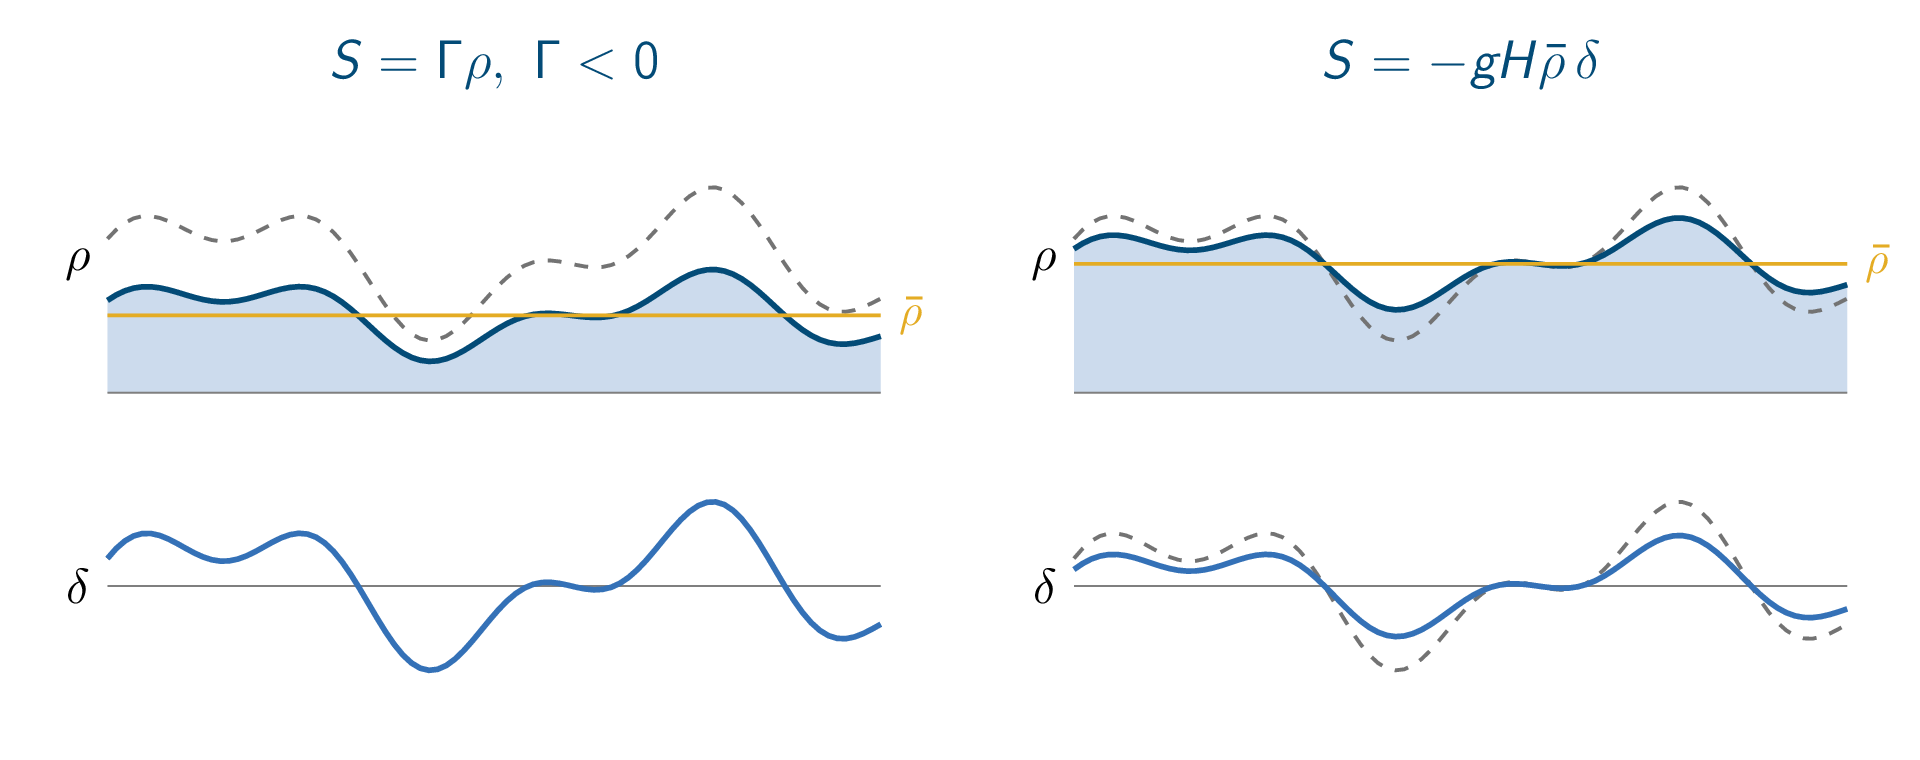
\includegraphics[width=\textwidth]{animacion_poster}}{animacion_toy.webm}
\end{frame}

% ####################################################################
% ##########  VERSIÓN VIEJA (propuesta, 18/nov/2026) — comentada  #####
% ####################################################################
% % ====================================================
% \section{Objetivos}
% % ====================================================
% 
% \begin{frame}{Objetivos}
%   \textbf{General:} estudiar la covarianza de los estimadores de la función
%   de correlación $\xi(r)$ en modelos de dilución de materia oscura, siguiendo
%   el enfoque de Wang \& Steele, con campos gaussianos.
% 
%   \vspace{0.6em}
%   \textbf{Objetivos ilustrativos:}
%   \begin{enumerate}
%     \item Resolver el crecimiento lineal $D_+$, $D_\Psi$ y $f_v=f+g$ para el
%       benchmark de dilución $g(z)$.
%     \item Generar realizaciones de campos gaussianos y catálogos con y sin
%       dilución ($g=0$ vs.\ $g\neq0$).
%     \item Medir $\hat\xi(r)$ y su matriz de covarianza a partir de las
%       realizaciones; compararla con la predicción gaussiana.
%     \item Explorar si la diferencia entre ambos modelos es significativa
%       frente al error estadístico.
%   \end{enumerate}
% \end{frame}
% 
% % ====================================================
% \section{Motivación}
% % ====================================================
% 
% \begin{frame}{Motivación}
%   \begin{columns}[T]
%     \begin{column}{0.55\textwidth}
%       \begin{itemize}
%         \item En $\Lambda$CDM plano, el $\Omega_m$ inferido de BAO de
%           \textbf{DESI DR2} es menor que el de \textbf{Planck} (CMB).
%         \item No es evidencia de intercambio de energía en el sector oscuro,
%           pero motiva preguntar si parte de lo atribuido a la energía oscura
%           viene de un cambio en la \alert{materia}.
%         \item Modelos con la misma expansión de fondo pueden tener
%           \emph{clustering} distinto $\Rightarrow$ las perturbaciones
%           rompen la degeneración.
%         \item ¿Es la señal detectable? Hace falta conocer la
%           \alert{covarianza} de los estimadores.
%       \end{itemize}
%     \end{column}
%     \begin{column}{0.42\textwidth}
%       \centering
%       \begin{tikzpicture}[x=70cm, y=1cm]
%         \draw[->] (0.27,0) -- (0.34,0) node[right, font=\small] {$\Omega_m$};
%         \foreach \x in {0.28,0.30,0.32}
%           \draw (\x,0.08) -- (\x,-0.08) node[below, font=\scriptsize] {\x};
%         % DESI DR2 BAO
%         \draw[myblue, very thick] (0.2975-0.0086,1.4) -- (0.2975+0.0086,1.4);
%         \fill[myblue] (0.2975,1.4) circle (2.5pt);
%         \node[myblue, font=\scriptsize, above] at (0.2975,1.5) {DESI DR2 BAO};
%         % Planck 2018
%         \draw[myred, very thick] (0.3153-0.0073,0.7) -- (0.3153+0.0073,0.7);
%         \fill[myred] (0.3153,0.7) circle (2.5pt);
%         \node[myred, font=\scriptsize, above] at (0.3153,0.8) {Planck 2018};
%       \end{tikzpicture}
% 
%       \vspace{0.3em}
%       {\scriptsize $\Omega_m = 0.2975\pm0.0086$ (DESI DR2)\\
%       $\Omega_m = 0.315\pm0.007$ (Planck 2018)}
%     \end{column}
%   \end{columns}
% \end{frame}
% 
% % ====================================================
% \section{Punto de partida}
% % ====================================================
% 
% \begin{frame}{Punto de partida}
%   \begin{columns}[T]
%     \begin{column}{0.5\textwidth}
%       \textbf{Continuidad modificada:}
%       \[
%         \dot\rho + 3H\rho + \nabla\!\cdot(\rho\,\dot{\mathbf{x}}) = S,
%         \qquad S = -g(t)H\bar\rho\,\delta
%       \]
%       \textbf{Crecimiento lineal} de la materia:
%       \[
%         \ddot D_+ + 2H(1+\Theta)\dot D_+
%         - \tfrac32\Omega_m H^2 (1+\Xi) D_+ = 0
%       \]
%       \vspace{-0.6em}
%       {\small $\Theta = g/2$, \ $\Xi = \Xi(g,\dot g)$; \ $g=0 \Rightarrow \Lambda$CDM.}
%     \end{column}
%     \begin{column}{0.47\textwidth}
%       \textbf{Efecto en $P(k)$ a orden lineal:}
%       \[
%         P_{\rm dil}(k) = \left[\frac{D_+^{\rm dil}}{D_+^{\Lambda{\rm CDM}}}\right]^2
%         P_{\Lambda{\rm CDM}}(k)
%       \]
%       \begin{itemize}
%         \item Solo suprime la amplitud: misma forma y mismo BAO.
%       \end{itemize}
%     \end{column}
%   \end{columns}
%   \begin{block}{}
%     \small Base: A.~Avilés \& J.~Ferrara, \textit{Dark Matter Dilution} (borrador).
%   \end{block}
% \end{frame}
% 
% % ====================================================
% \section{Entradas}
% % ====================================================
% 
% \begin{frame}{Entradas: modelo de juguete}
%   \begin{itemize}
%     \item \textbf{Benchmark del borrador:} fondo $\Lambda$CDM plano,
%       $\Omega_{m0}=0.3$, con
%       \[
%         g(z) = \frac{g_0}{2}\left[1 - \tanh\!\left(\frac{z-z_t}{\Delta z}\right)\right],
%         \quad g_0=0.2,\; z_t=2,\; \Delta z=0.2 .
%       \]
%     \item \textbf{Espectro lineal} $P_L(k)$ (CAMB, como en la práctica 04),
%       reescalado con $D_+$ de cada modelo.
%     \item \textbf{Campos gaussianos hechos a mano} en una caja periódica (FFT):
%       $\delta_0(\mathbf{k}) \to \delta^{(1)},\ \Psi^{(1)},\ \mathcal{M}^{(1)}$.
%     \item \textbf{Catálogos:} partículas desplazadas (Zel'dovich con $D_\Psi$)
%       con peso $\mathcal{M}$; catálogos aleatorios para los estimadores.
%     \item Muchas realizaciones con semillas distintas $\Rightarrow$ covarianza muestral.
%   \end{itemize}
% \end{frame}
% 
% % ====================================================
% \section{Salidas}
% % ====================================================
% 
% \begin{frame}{Salidas esperadas}
%   \alert{Por definir con más detalle}; la idea es observar:
%   \begin{itemize}
%     \item $\hat\xi(r)$ (Landy--Szalay y otros) para $g=0$ y $g\neq0$.
%     \item Matrices de covarianza y de correlación entre bins de $r$.
%     \item Comparación entre covarianza muestral y predicción gaussiana
%       (Wang \& Steele).
%     \item Cómo cambian el ruido y la covarianza con el número de
%       realizaciones, de aleatorios y el ancho de bin.
%   \end{itemize}
% \end{frame}
% 
% % ====================================================
% \section{Plan de implementación}
% % ====================================================
% 
% \begin{frame}{Plan de implementación}
%   \centering
%   \begin{tikzpicture}[
%       box/.style={draw=myblue, thick, rounded corners, fill=myblue!8,
%         align=center, minimum height=1.4cm, text width=2.6cm, font=\small},
%       arr/.style={-{Stealth}, thick, myblue}]
%     \node[box] (a) {\textbf{1.} Crecimiento\\$D_+,\ D_\Psi$};
%     \node[box, right=0.5cm of a] (b) {\textbf{2.} Campos\\gaussianos};
%     \node[box, right=0.5cm of b] (c) {\textbf{3.} Medir\\$\hat\xi(r)$};
%     \node[box, right=0.5cm of c, fill=mygreen!10, draw=mygreen] (d)
%       {\textbf{4.} Covarianza};
%     \draw[arr] (a) -- (b); \draw[arr] (b) -- (c); \draw[arr] (c) -- (d);
%     \draw[arr, myorange] (c.south) to[out=-60, in=-120, looseness=1.2]
%       node[below, font=\small] {$N$ realizaciones} (b.south);
%   \end{tikzpicture}
% 
%   \vspace{1em}
%   \raggedright\small
%   Se compara $g=0$ vs.\ $g\neq0$, y la covarianza muestral vs.\ la gaussiana.\\[0.4em]
%   \alert{Por investigar:} la covarianza de Wang \& Steele con pesos $\mathcal{M}$.
% \end{frame}
% 
% % ====================================================
% \section{Bibliografía}
% % ====================================================
% 
% \begin{frame}{Bibliografía}
%   \begin{block}{Trabajo base}
%     \small
%     \begin{itemize}
%       \item A.~Avilés \& J.~Ferrara, \textit{Dark Matter Dilution: A Two-Field Lagrangian
%         Perturbation Theory of Large-Scale Structure}, borrador (en preparación).
%     \end{itemize}
%   \end{block}
%   \vspace{0.3em}
%   \begin{exampleblock}{Semilla}
%     \small
%     \begin{itemize}
%       \item DESI Collaboration (M.~Abdul-Karim \etal), \textit{DESI DR2 Results II:
%         Measurements of BAO and Cosmological Constraints}, arXiv:2503.14738.
%       \item Planck Collaboration (N.~Aghanim \etal), \textit{Planck 2018 results.
%         VI. Cosmological parameters}, A\&A \textbf{641} (2020) A6, arXiv:1807.06209.
%     \end{itemize}
%   \end{exampleblock}
% \end{frame}
% 
% % ---- cierre: con fondo de sección ----
% \section{¡Gracias! \texorpdfstring{\\[0.4em]}{} {\normalsize ¿Preguntas y comentarios?}}
% \sectionframe

\end{document}
